\chapter{Hướng dẫn chạy}
\label{sec:contribute}
\begin{enumerate}
    \item Vô Google Drive, tạo thư mục 'colab/demand-forecast' và up file 'gld.csv' trong thư mục 'data' lên
    \begin{figure}[h]
        \center{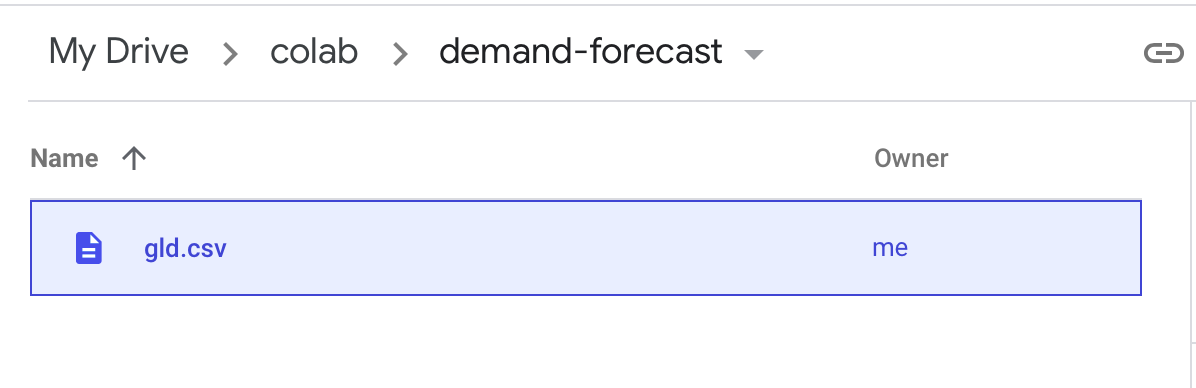
\includegraphics[width=6cm]
        {figure/googledrive.png}}
    \end{figure}
    \item Vô Google Colab. Chọn File -> Upload notebook, up file Last90dayValidation.ipynb hoặc WalkForwaldValidation.ipynb lên Google Colab.
    \begin{figure}[h]
        \center{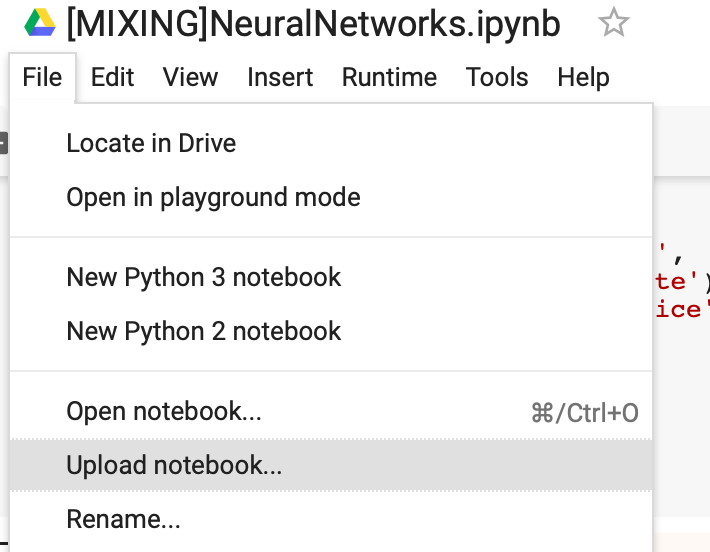
\includegraphics[width=6cm]
        {figure/upload.png}}
    \end{figure}
    \item Chọn Runtime -> Change runtime type. Trong mục Hardware accelerator, chọn GPU. Nhấn Save. 
    \begin{figure}[!h]
        \center{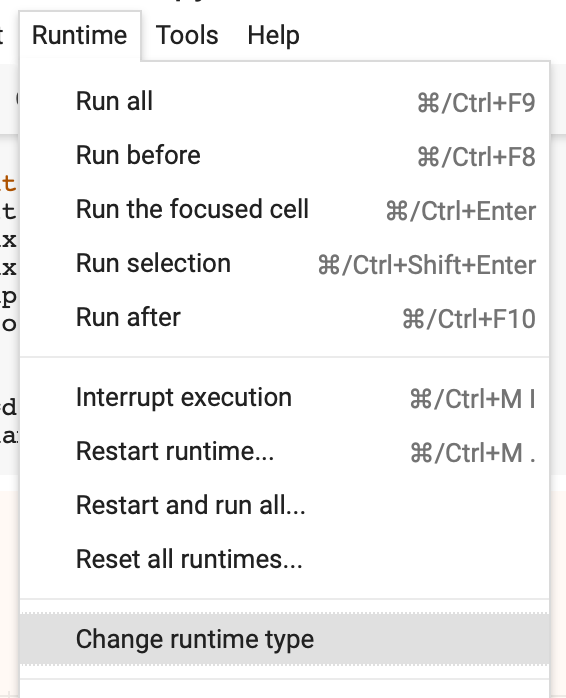
\includegraphics[width=6cm]
        {figure/changegpu.png}}
    \end{figure}
    \begin{figure}[h]
        \center{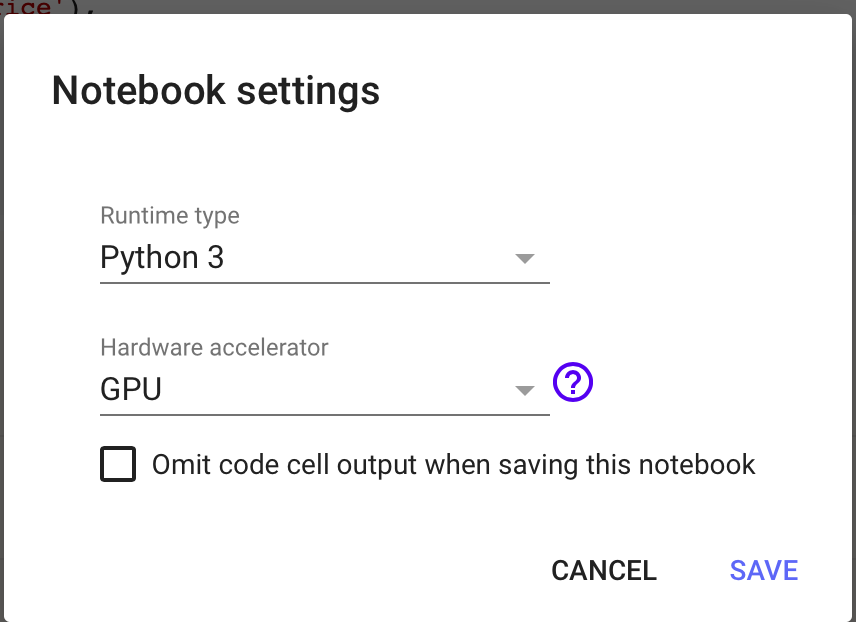
\includegraphics[width=6cm]
        {figure/changegpu2.png}}
    \end{figure}
    \clearpage
    \item Chọn Runtime -> Run all để chạy. Lưu ý, trong lúc chạy sẽ thông báo truy cập vào link Google Drive để cấp quyền truy cập vào Google Drive ở cell thứ 1. 
    \begin{figure}[h]
        \center{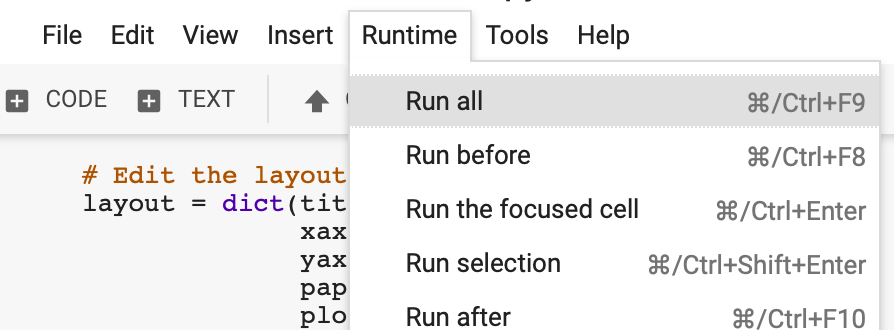
\includegraphics[width=8cm]
        {figure/runall.png}}
    \end{figure}
    \begin{figure}[h]
        \center{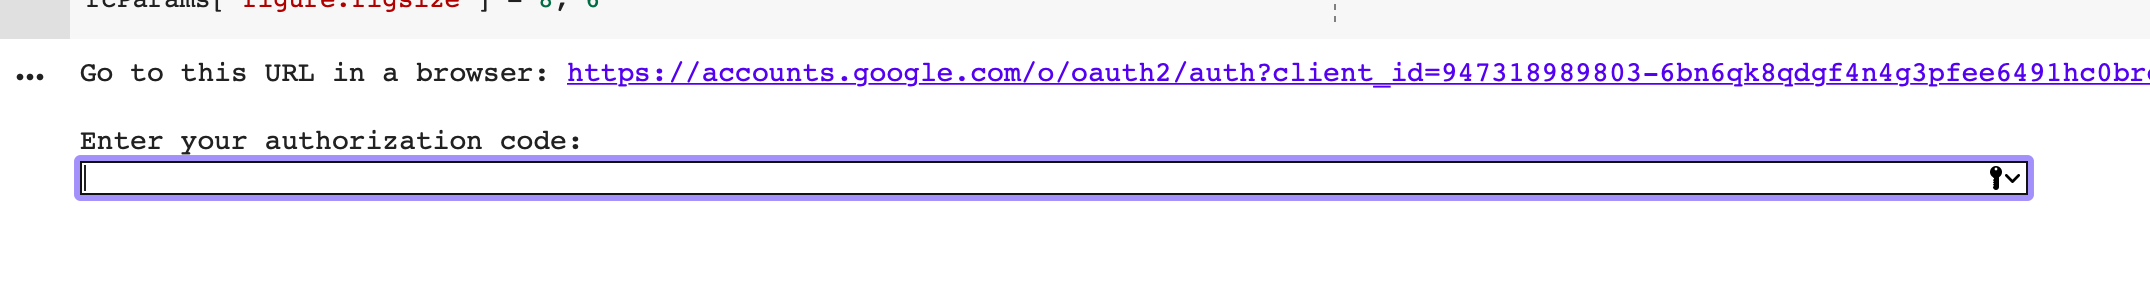
\includegraphics[width=16cm]
        {figure/googleauth.png}}
    \end{figure}
    \item Kết quả
    \begin{figure}[h]
        \center{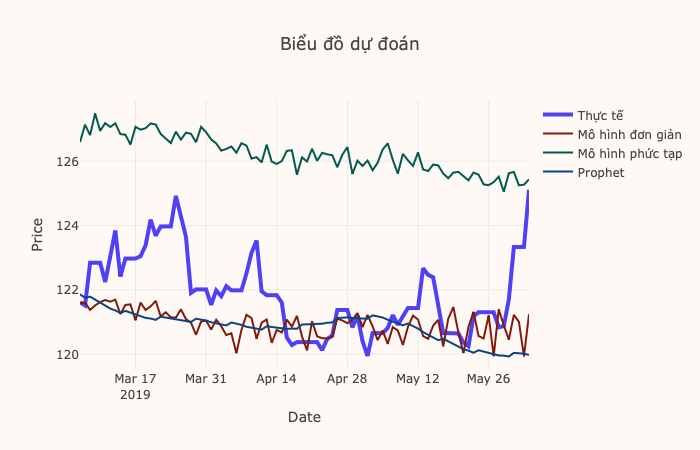
\includegraphics[width=12cm]
        {figure/result.png}}
    \end{figure}
\end{enumerate}
